%----------------------------------------------------------------------------------------
%	PACKAGES AND OTHER DOCUMENT CONFIGURATIONS
%----------------------------------------------------------------------------------------

\documentclass[paper=a4, fontsize=10pt]{scrartcl} % A4 paper and 11pt font size

\usepackage[T1]{fontenc}
\usepackage{fourier}
\usepackage[english]{babel}
\usepackage{amsmath,amsfonts,amsthm}
\usepackage{graphicx}
\usepackage{caption}
\usepackage{subcaption}
\usepackage{hyperref}

\usepackage{sectsty} % Allows customizing section commands
\allsectionsfont{\centering \normalfont\scshape} % Make all sections centered, the default font and small caps

\usepackage{fancyhdr} % Custom headers and footers

\fancyhead{} % No page header - if you want one, create it in the same way as the footers below
\fancyfoot[R]{\thepage} % Page numbering for right footer
\renewcommand{\headrulewidth}{0pt} % Remove header underlines
\renewcommand{\footrulewidth}{0pt} % Remove footer underlines

\numberwithin{equation}{section} % Number equations within sections (i.e. 1.1, 1.2, 2.1, 2.2 instead of 1, 2, 3, 4)
\numberwithin{figure}{section} % Number figures within sections (i.e. 1.1, 1.2, 2.1, 2.2 instead of 1, 2, 3, 4)

%----------------------------------------------------------------------------------------
%	TITLE SECTION
%----------------------------------------------------------------------------------------

\newcommand{\horrule}[1]{\rule{\linewidth}{#1}} % Create horizontal rule command with 1 argument of height

\title{	
\normalfont \normalsize 
\horrule{0.5pt} \\[0.4cm] % Thin top horizontal rule
\huge E-Gym Programming Assignment \\ % The assignment title
\horrule{2pt} \\[2.9cm] % Thick bottom horizontal rule
}

\author{Taner GUNGOR} % Your name

\date{\normalsize\today} % Today's date or a custom date

\begin{document}

\maketitle % Print the title

%----------------------------------------------------------------------------------------
%	PROBLEM 1
%----------------------------------------------------------------------------------------

\section{Problem definition}

With this assignment three jpeg images numbered from one to three are received. There is a white sheet of paper folded in half in each of the images. The task is to write an application that finds the center of the sheet of paper. Finding the paper gets progressively trickier. The application should take an input file name as command-line argument and search the image file with that name. After finding the center of the sheet of paper, a new image with a red dot in the center of the sheet of paper saved under a new name.

%----------------------------------------------------------------------------------------

\section{Methodology}

There are many techniques to extract the white sheet of paper from the images given. In this section the whole process, where the basic image processing algorithms are used, is explained in a simple way.
 
\subsection{Thresholding}

Thresholding is the simplest method of image segmentation. From a gray-scale image, thresholding can be used to create binary images. The simplest thresholding methods replace in an image with a black pixel if the image intensity $I_{i, j}$ is less than some fixed constant T (that is, $I_{i, j} < T$ ), or a white pixel if the image intensity is greater than that constant. The figure \ref{fig:thresholding} shows the thresholding results.

\begin{figure}
	\centering
	\begin{subfigure}[b]{0.35\textwidth}
		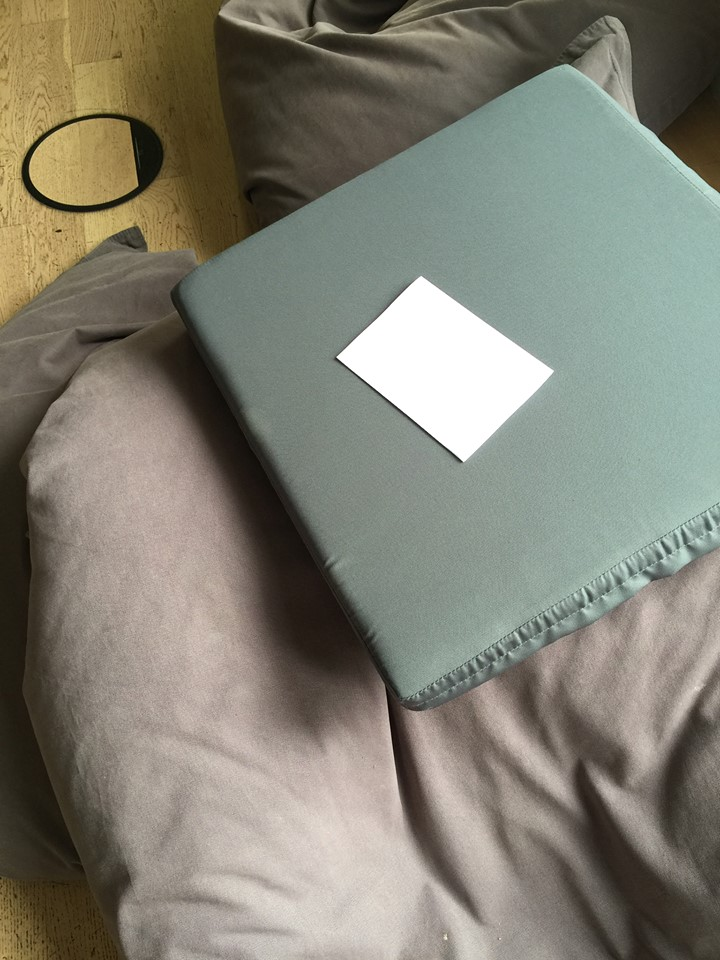
\includegraphics[width=\textwidth]{01}
		\caption{Input - 1}
		\label{fig:input_01}
	\end{subfigure}
	~ 
	\begin{subfigure}[b]{0.35\textwidth}
		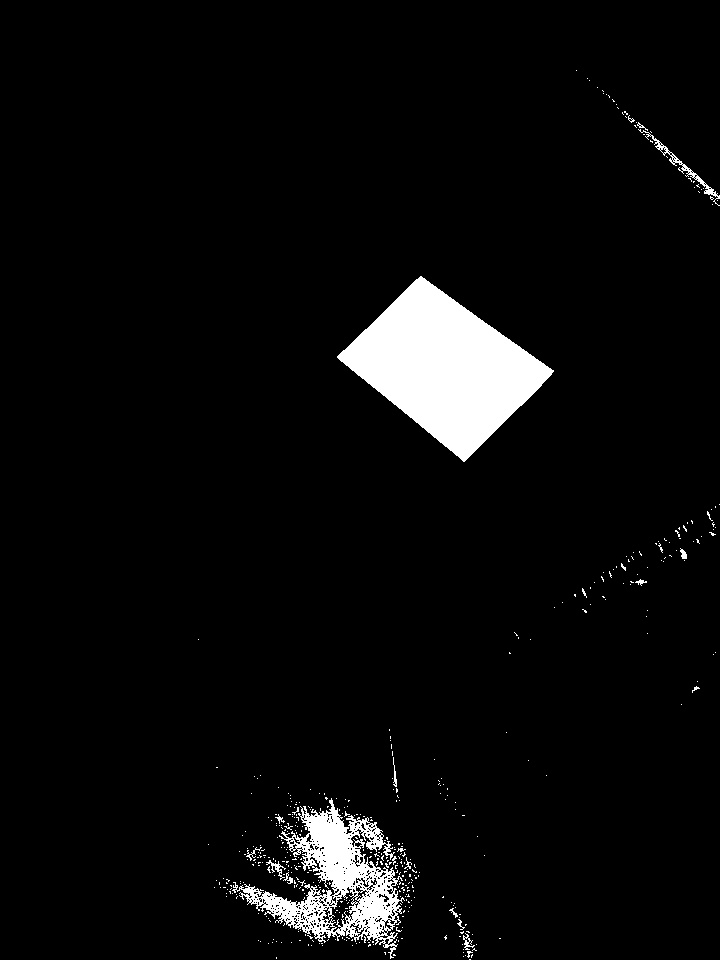
\includegraphics[width=\textwidth]{binary_01}
		\caption{Binary output - 1}
		\label{fig:binary_output_01}
	\end{subfigure}
	
	\centering
	\begin{subfigure}[b]{0.35\textwidth}
		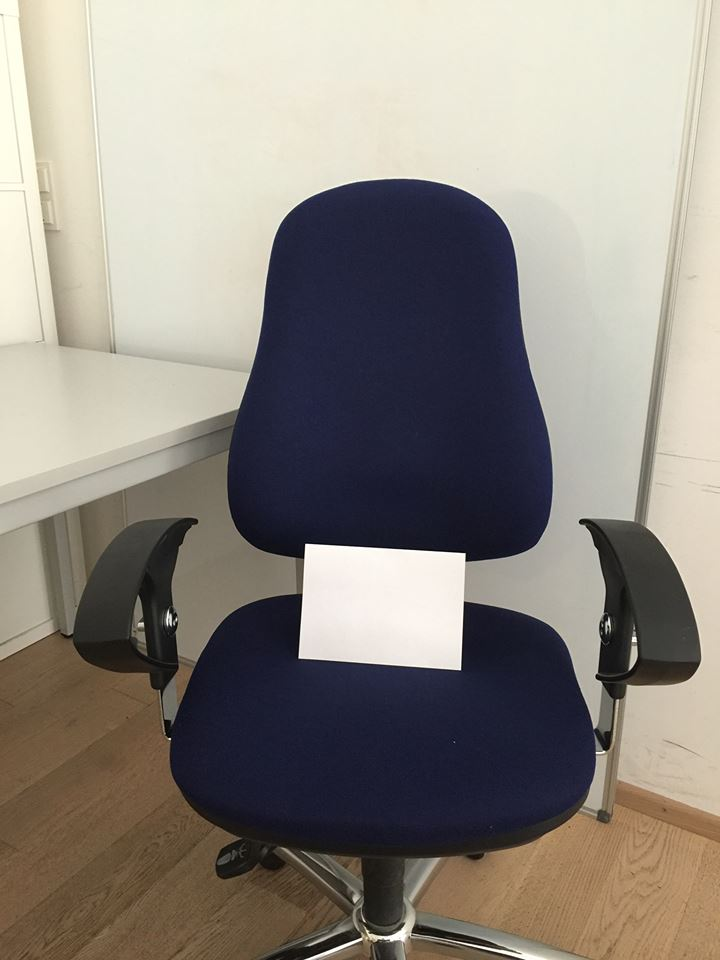
\includegraphics[width=\textwidth]{02}
		\caption{Input - 2}
		\label{fig:input_02}
	\end{subfigure}
	~ 
	\begin{subfigure}[b]{0.35\textwidth}
		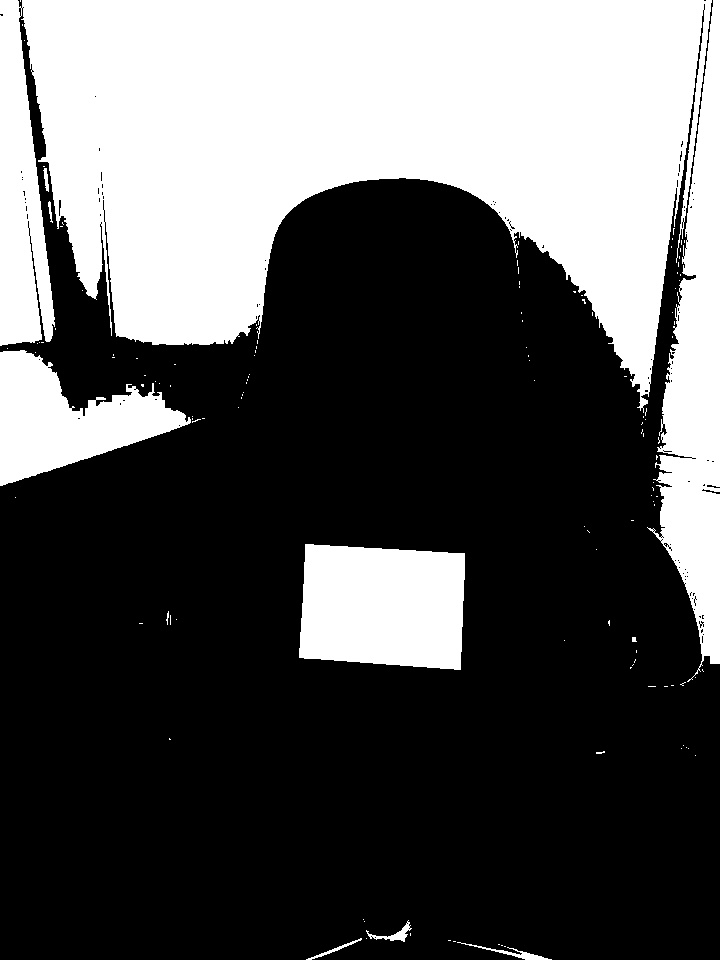
\includegraphics[width=\textwidth]{binary_02}
		\caption{Binary output - 2}
		\label{fig:binary_output_02}
	\end{subfigure}

	\centering
	\begin{subfigure}[b]{0.35\textwidth}
		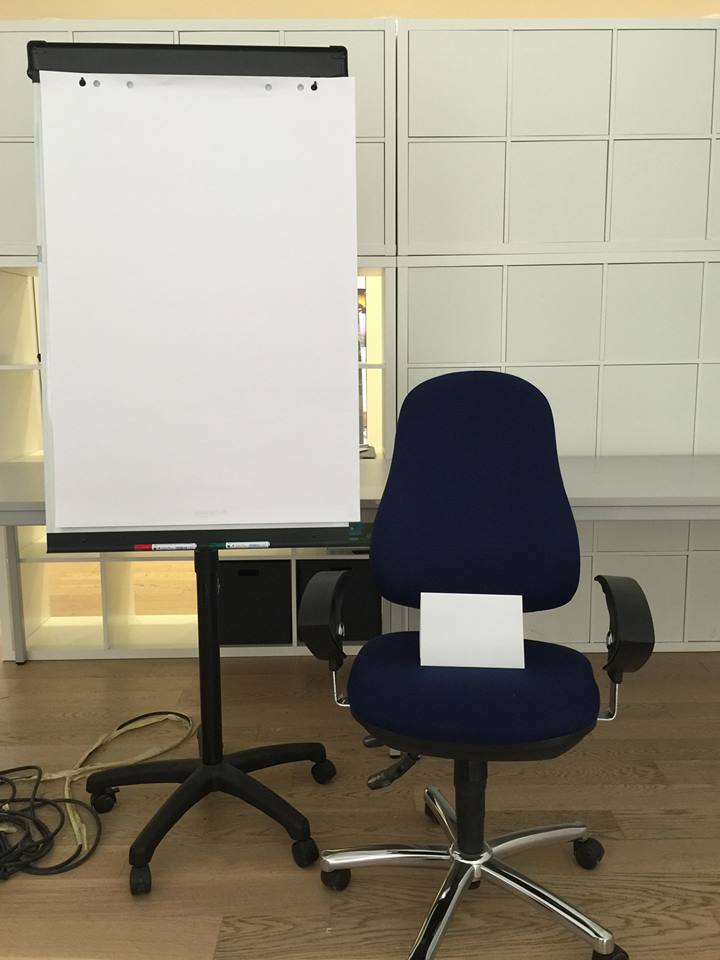
\includegraphics[width=\textwidth]{03}
		\caption{Input - 3}
		\label{fig:input_03}
	\end{subfigure}
	~ 
	\begin{subfigure}[b]{0.35\textwidth}
		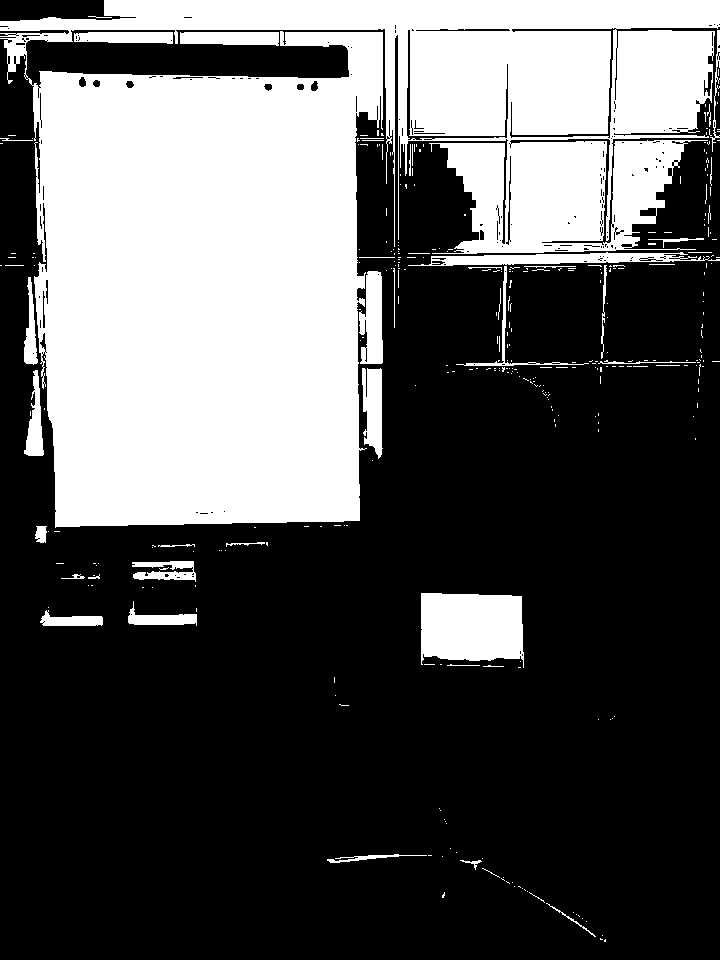
\includegraphics[width=\textwidth]{binary_03}
		\caption{Binary output - 3}
		\label{fig:binary_output_03}
	\end{subfigure}

	\caption{The outputs for each input image}
	\label{fig:thresholding}
\end{figure}

\subsection{Dilation}
Dilation is one of the basic operations in mathematical morphology. The dilation operation usually uses a structuring element for probing and expanding the shapes contained in the input image. The figure \ref{fig:dilation} shows the dilation results.

\begin{figure}[!ht]
	\centering
	\begin{subfigure}[b]{0.275\textwidth}
		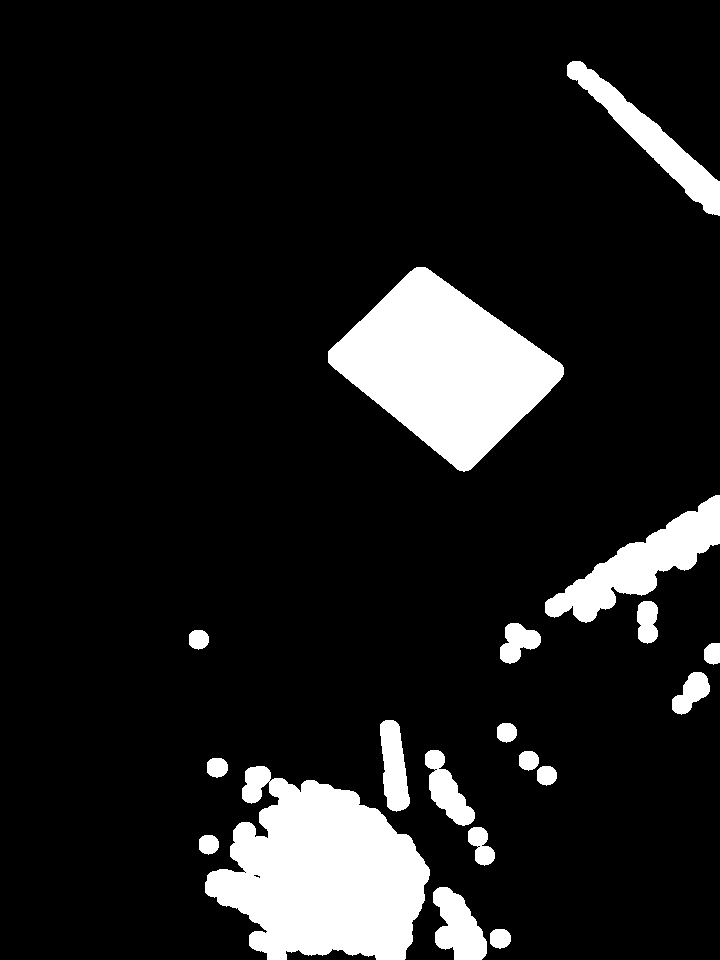
\includegraphics[width=\textwidth]{dilation_01}
		\caption{Dilation output - 1}
		\label{fig:dilation_output_01}
	\end{subfigure}
	~ 
	\begin{subfigure}[b]{0.275\textwidth}
		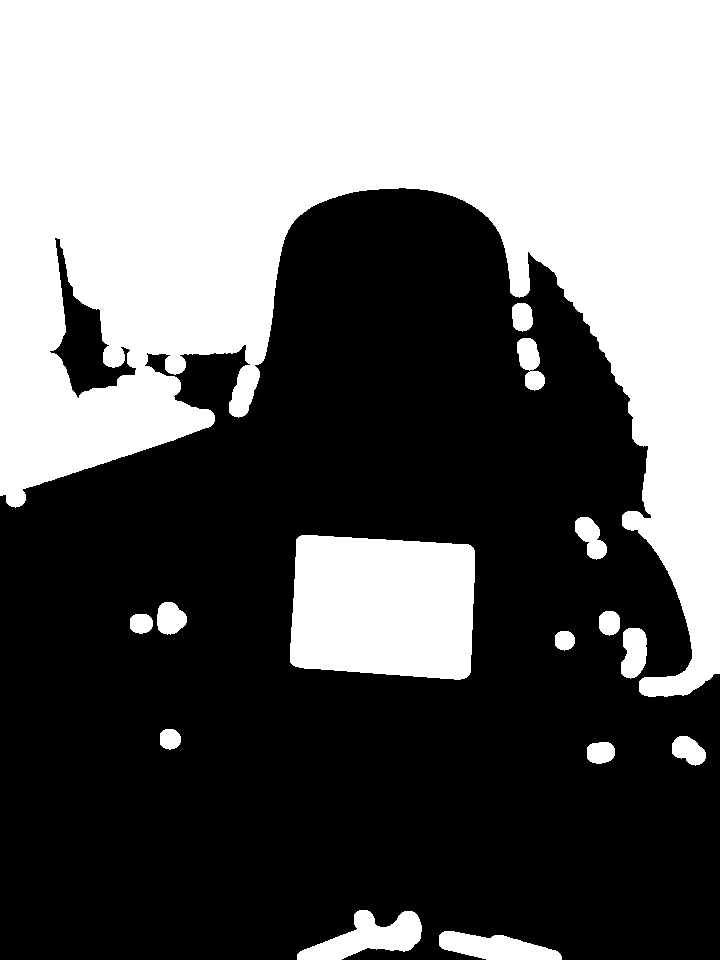
\includegraphics[width=\textwidth]{dilation_02}
		\caption{Dilation output - 2}
		\label{fig:dilation_output_02}
	\end{subfigure}
	~ 
	\begin{subfigure}[b]{0.275\textwidth}
		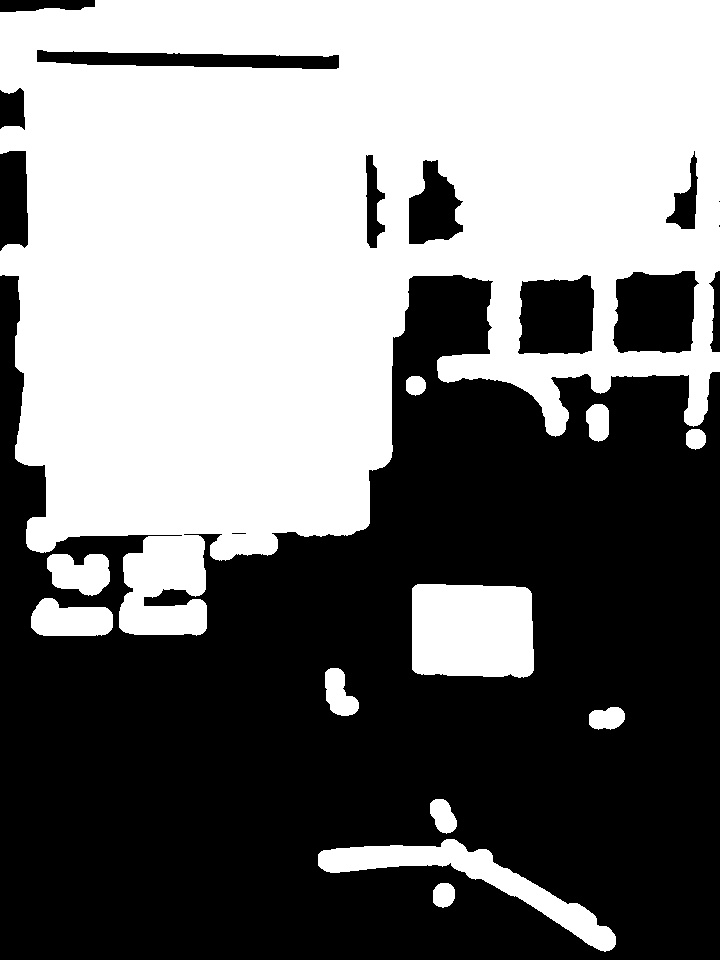
\includegraphics[width=\textwidth]{dilation_03}
		\caption{Dilation output - 3}
		\label{fig:dilation_output_03}
	\end{subfigure}
	\caption{The dilation outputs for each binary image}
	\label{fig:dilation}
\end{figure}

\subsection{Suppressing the structures connected to image border}
The next step is suppressing the structures that are connected to the image border. The figure \ref{fig:s_dilation} shows the results.

\begin{figure}[!ht]
	\centering
	\begin{subfigure}[b]{0.275\textwidth}
		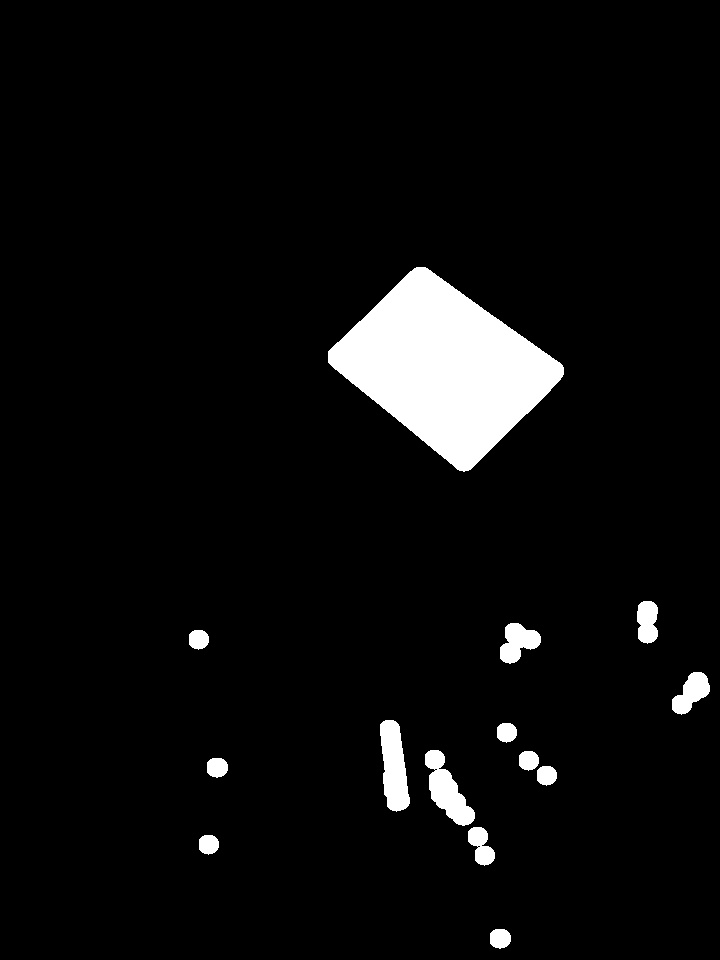
\includegraphics[width=\textwidth]{s_dilation_01}
		\caption{Output - 1}
		\label{fig:s_dilation_output_01}
	\end{subfigure}
	~ 
	\begin{subfigure}[b]{0.275\textwidth}
		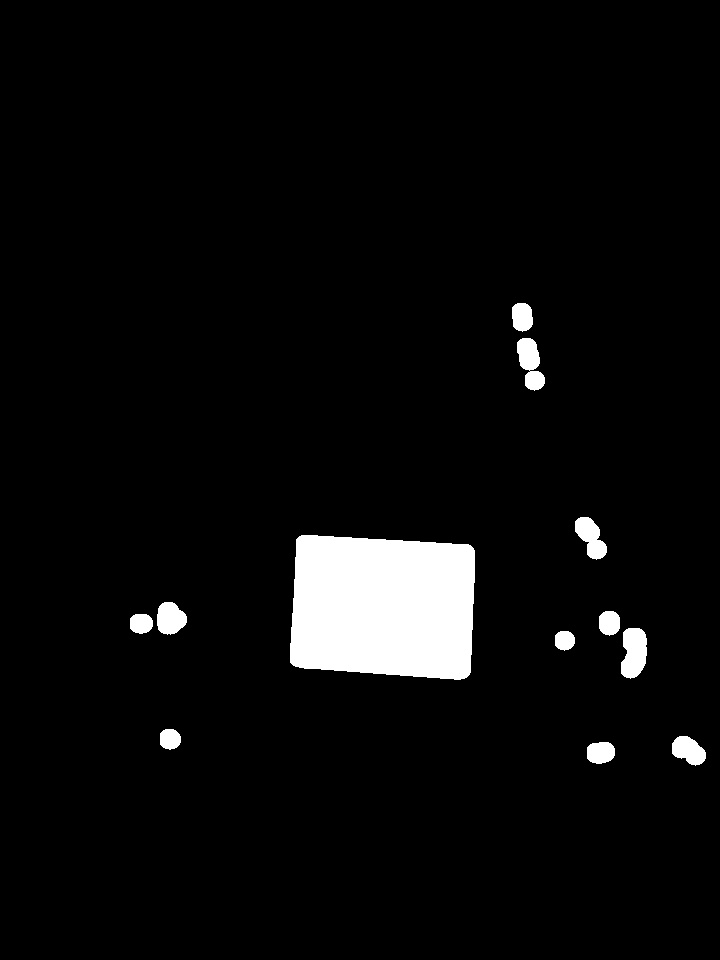
\includegraphics[width=\textwidth]{s_dilation_02}
		\caption{Output - 2}
		\label{fig:s_dilation_output_02}
	\end{subfigure}
	~ 
	\begin{subfigure}[b]{0.275\textwidth}
		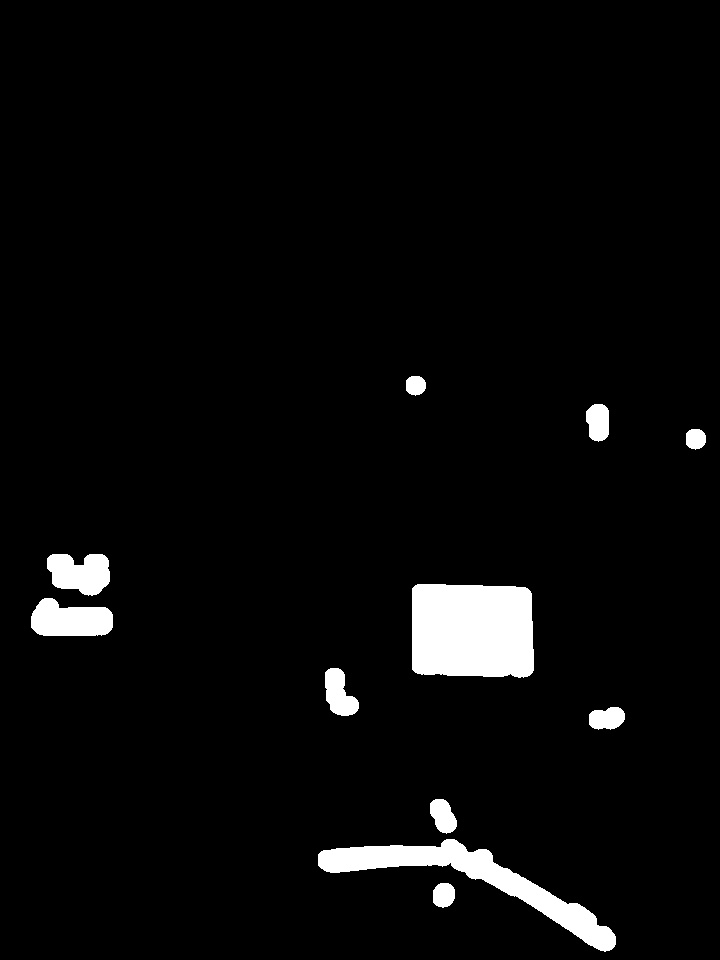
\includegraphics[width=\textwidth]{s_dilation_03}
		\caption{Output - 3}
		\label{fig:s_dilation_output_03}
	\end{subfigure}
	\caption{Suppressing the structures connected to image border for each dilated image}
	\label{fig:s_dilation}
\end{figure}

\subsection{Erosion}
Erosion is another fundamental operations in morphological image processing from which all other morphological operations are based. The basic effect of the operator on a binary image is to erode away the boundaries of regions of foreground pixels. Thus areas of fore-ground pixels shrink in size, and holes within those areas become larger. The figure \ref{fig:erosion} shows the erosion results.

\begin{figure}[!ht]
	\centering
	\begin{subfigure}[b]{0.275\textwidth}
		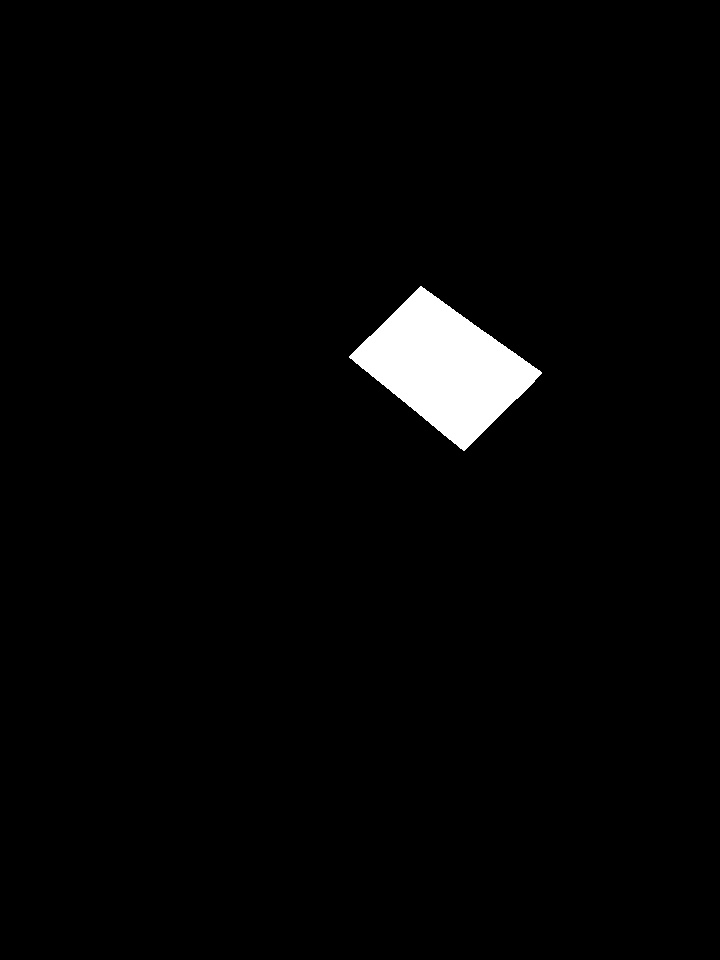
\includegraphics[width=\textwidth]{erosion_01}
		\caption{Erosion output - 1}
		\label{fig:erosion_01}
	\end{subfigure}
	~ 
	\begin{subfigure}[b]{0.275\textwidth}
		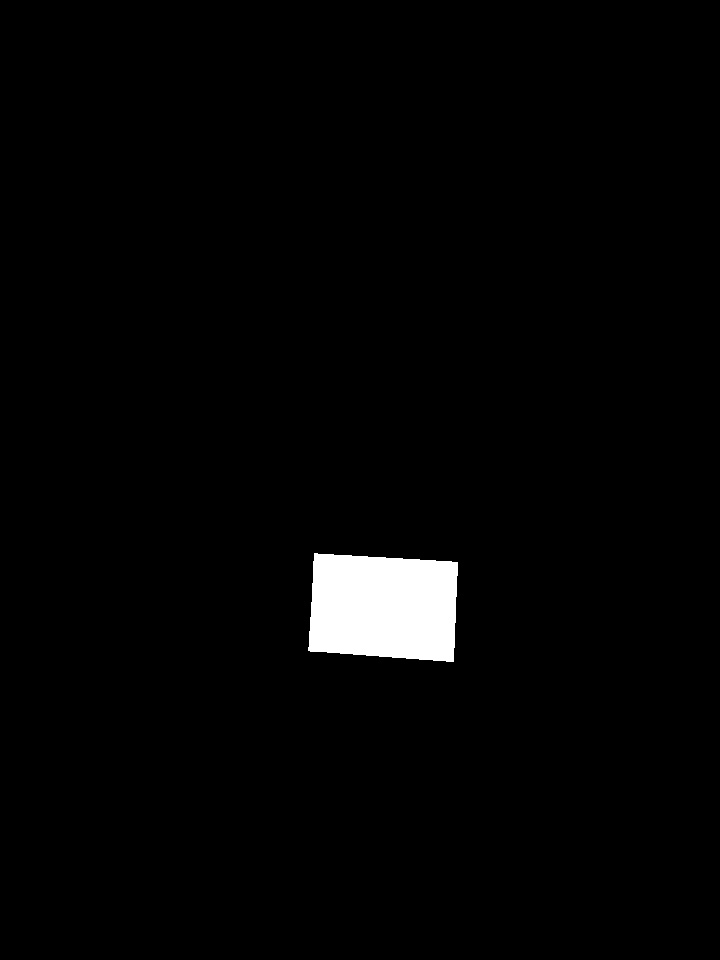
\includegraphics[width=\textwidth]{erosion_02}
		\caption{Erosion output - 2}
		\label{fig:erosion_02}
	\end{subfigure}
	~ 
	\begin{subfigure}[b]{0.275\textwidth}
		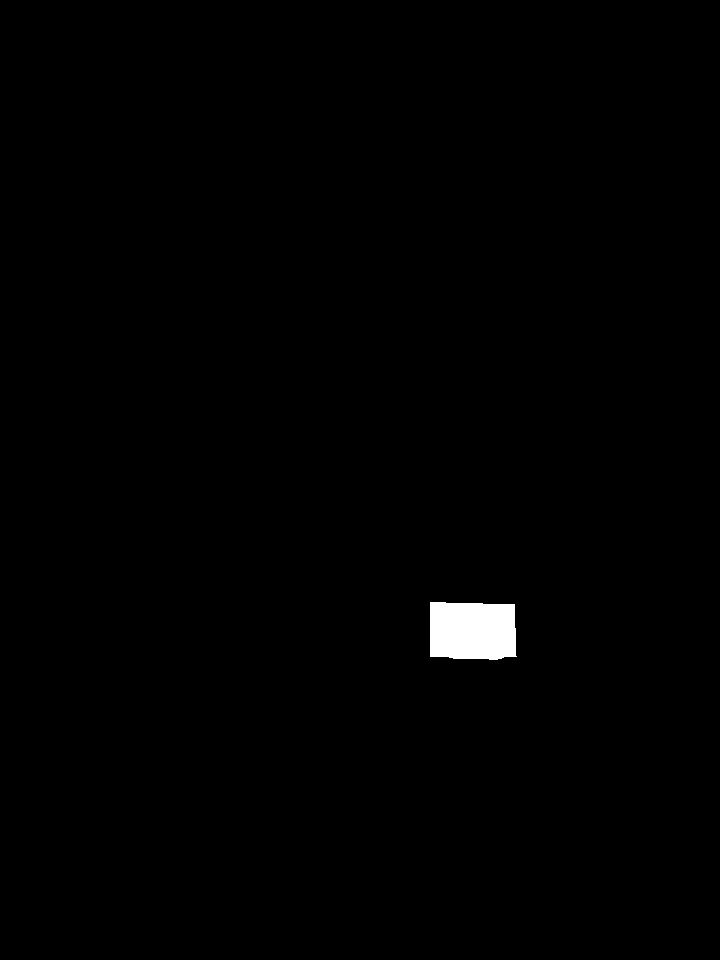
\includegraphics[width=\textwidth]{erosion_03}
		\caption{Erosion output - 3}
		\label{fig:erosiont_03}
	\end{subfigure}
	\caption{The outputs of erosion for each dilated image}
	\label{fig:erosion}
\end{figure}

\subsection{Finding the center of the mass}
Image moments help us to calculate the center of mass of the object. In order to obtain image moments, \textit{findContours} method is used. After finding the center of mass of the object, a new image with a dot in the center of the mass of the object is saved under a new name. The figure \ref{fig:results} shows the results.

\begin{figure}[!ht]
	\centering
	\begin{subfigure}[b]{0.25\textwidth}
		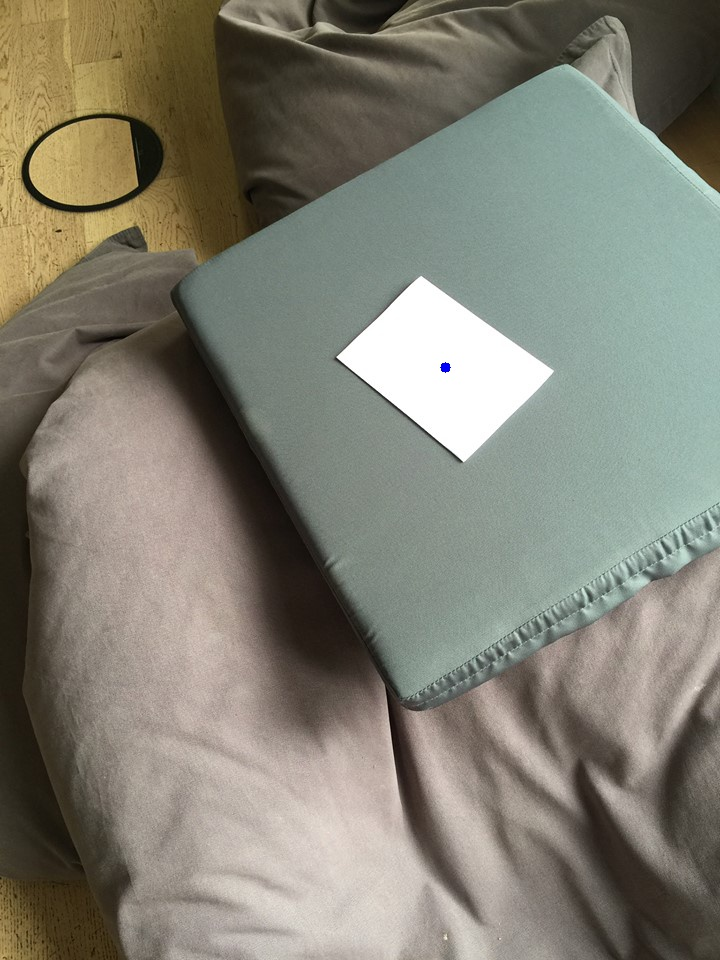
\includegraphics[width=\textwidth]{output_01}
		\caption{Output - 1}
		\label{fig:output_01}
	\end{subfigure}
	~ 
	\begin{subfigure}[b]{0.25\textwidth}
		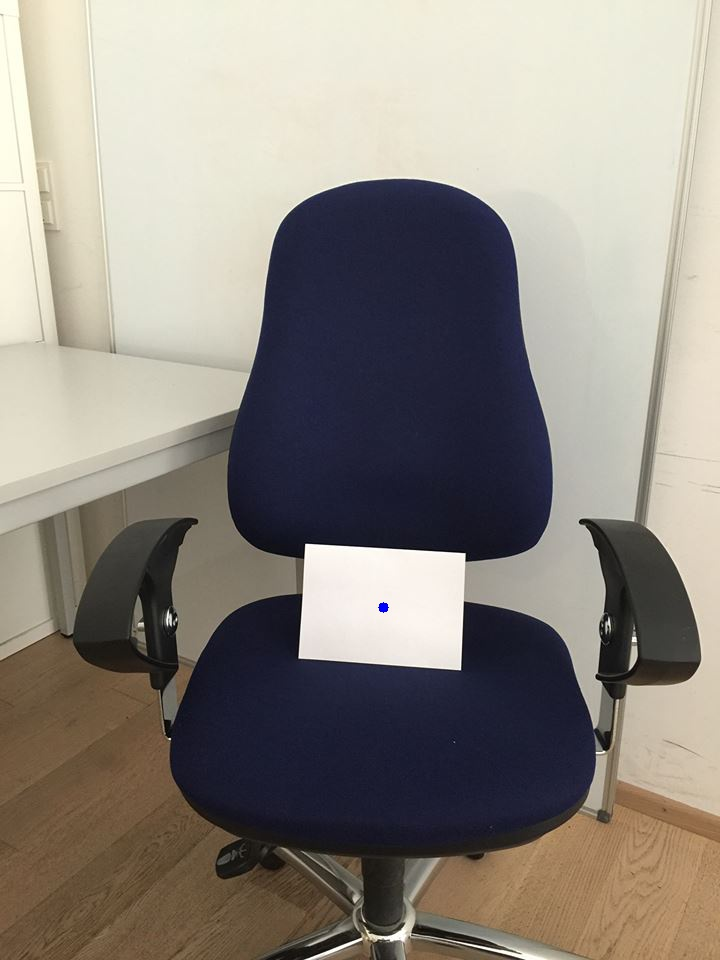
\includegraphics[width=\textwidth]{output_02}
		\caption{Output - 2}
		\label{fig:output_02}
	\end{subfigure}
	~ 
	\begin{subfigure}[b]{0.25\textwidth}
		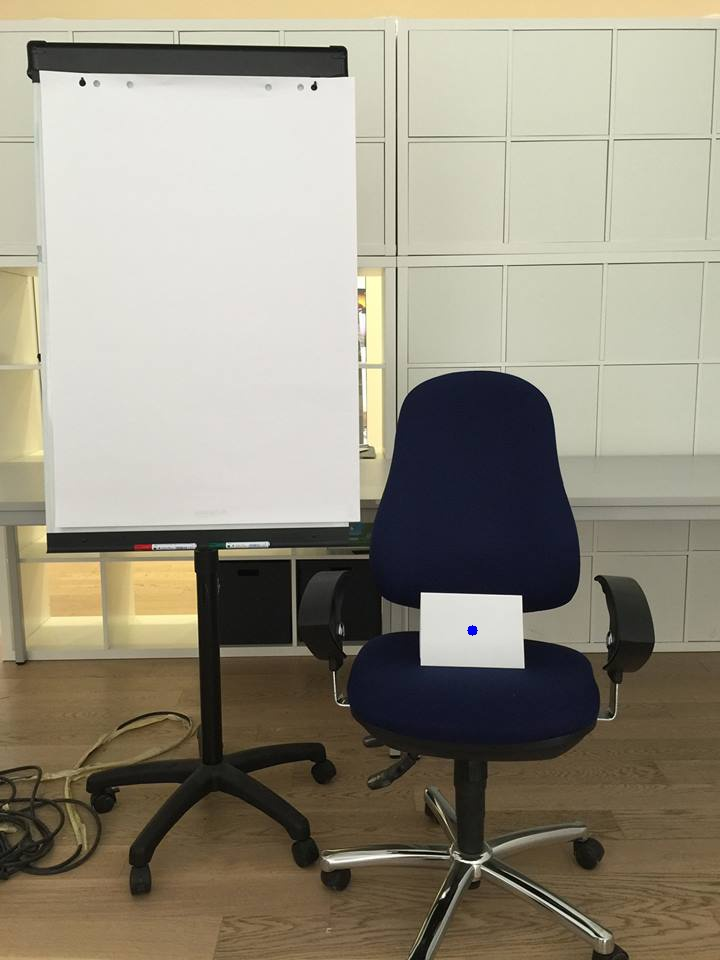
\includegraphics[width=\textwidth]{output_03}
		\caption{Output - 3}
		\label{fig:output_03}
	\end{subfigure}
	\caption{The outputs for each input image}
	\label{fig:results}
\end{figure}

%----------------------------------------------------------------------------------------

\section{Results}

Windows 8.1 Pro 64-bit operating system is used for development process. The task is first implemented in Matlab 2015b. Then it is successfully coded by using Qt Creator 4.0.1. QT version is Qt 5.7.0 (MSVC 2015, 64-bit) and the compiler is Microsoft Visual C++ Compiler 14.0 (amd64). The figure \ref{fig:results} shows the output images for each input image.

\subsection{Limitations}

The algorithm explained above is highly related with the illumination. Let us say if the color of the paper is not white, then it will not work properly because of the threshold process. Another problem is that if the paper is connected to the image border, the algorithm will delete it before the erosion process. For these three images, algorithm is working well. But for the cases explained above, it may not work well.

\subsection{Possible Solutions}

There are some solutions to the problems explained above. Instead of using basic image processing algorithms, we can use some advance techniques such as hough transform or key-point descriptors and detectors. There are some useful links for hough transform in the following:

\begin{itemize}
	\item \href{http://www.imagemagick.org/discourse-server/viewtopic.php?t=25476}{Link-1}
	\item \href{http://stackoverflow.com/questions/10533233/opencv-c-obj-c-advanced-square-detection}{Link-2}
\end{itemize}

But for the last image, it might fail. Because there are many lines in the background. The second possible solution might be using a key-point descriptors and detectors like Scale-invariant feature transform (SIFT). There is a useful link below:

\begin{itemize}
	\item \href{http://opencv-python-tutroals.readthedocs.io/en/latest/py_tutorials/py_feature2d/py_feature_homography/py_feature_homography.html}{Link-1}
\end{itemize}

However, these two techniques are computationally expensive and especially SIFT is used for detecting much more complicated objects instead of just white paper.

%----------------------------------------------------------------------------------------

\end{document}